\documentclass[a4paper,10pt]{article}
\usepackage{polski}
\usepackage[utf8]{inputenc}
\usepackage{array,floatflt,textcomp,graphicx,longtable}
%custom margins
\usepackage[left=2.5cm, top=2.5cm, bottom=3cm, right=2cm, foot=2cm, head=0.5cm]{geometry}
\usepackage{fancyhdr}
\usepackage[bookmarks=true, pdftex]{hyperref}

%styl nagłowków
\pagestyle{fancy} 
\parindent 2cm 

%opening
\title{Analiza obiektowa}
\author{3@KASK}

\begin{document}
\bibliographystyle{plain}


\maketitle


\begin{center}
%budowanie tabeli
\begin{longtable}{|p{7cm}|p{7cm}|}
\hline
Symbol projektu: & Opiekun projektu:   \tabularnewline 
3@KASK & mgr inż. Tomasz Boiński    \tabularnewline \hline
\multicolumn{2}{|l|}{Nazwa Projektu: } \tabularnewline
\multicolumn{2}{|l|}{Wizualizacja grafów za pomocą biblioteki Prefuse } \tabularnewline 
\hline
\multicolumn{2}{l}{ } \tabularnewline %pusta linijka
\hline 
Nazwa Dokumentu: & Nr wersji:   \tabularnewline 
Analiza obiektowa & 0.0 \tabularnewline \hline
Odpowiedzialny za dokument: & Data pierwszego sporządzenia:   \tabularnewline 
Piotr Kunowski & 23 maja 2009 \tabularnewline \hline
Przeznaczenie: & Data ostatniej aktualizacji:   \tabularnewline 
DLA KLIENTA & \today \tabularnewline \hline
\end{longtable}
\end{center}


\begin{center}
\begin{longtable}{|c|p{4cm}|c|c|c|}
\multicolumn{5}{c}{\textbf{Historia dokumentu}} \tabularnewline \hline
\textbf{Wersja} & \textbf{Opis modyfikacji} & \textbf{Rozdział/strona} & \textbf{Autor modyfikacji} & \textbf{Data} \tabularnewline \hline 
1 & Stworzenie & wszystkie & Grupa projektowa & 23.05.09 \tabularnewline \hline

\end{longtable}
\end{center}


\newpage
\tableofcontents
\newpage

\section{Pakiety}

\subsection{Diagram}
 \scalebox{0.70}{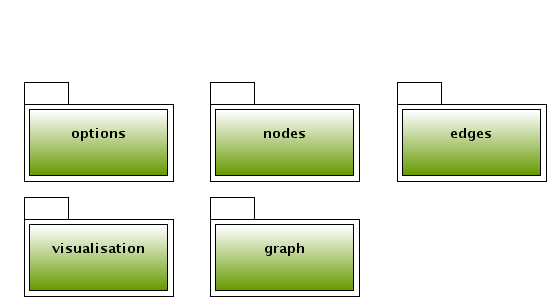
\includegraphics{./modelowanie/OV_UML/PackageDiagram.png}}


\subsection{Opis pakietów}


\begin{center}
\begin{longtable}{|m{3cm}|m{9cm}|} \hline

P001 & options\\ \hline
Opis: & Pakiet zawierający klasy z polami opisującymi różne (modyfikowalne) ustawienia wizualizacji takie jak: kolory, grubość linii itp.     \\ \hline
Interfejsy: &     \\ \hline
Realizowane wymagania: & WF002, WF001, WI004 \\ \hline
Priorytet: & średnio ważne \\ \hline

\multicolumn{2}{c}{} \\
 \hline

P002 & nodes\\ \hline
Opis: & Pakiet z klasami odpowiedzialnymi za wizualizację i przechowywanie danych o wierzchołkach.    \\ \hline
Interfejsy: &     \\ \hline
Realizowane wymagania: & WF004, WF005, WF006, WF007, WI004 \\ \hline
Priorytet: & bardzo ważne \\ \hline

\multicolumn{2}{c}{} \\
 \hline

P003 & edges\\ \hline
Opis: & Pakiet z klasami odpowiedzialnymi za wizualizację i przechowywanie danych o krawędziach.    \\ \hline
Interfejsy: &     \\ \hline
Realizowane wymagania: & WF006, WF007, WI004 \\ \hline
Priorytet: & bardzo ważne \\ \hline

\multicolumn{2}{c}{} \\
 \hline

P004 & visualization\\ \hline
Opis: & Zawiera dodatkowe klasy przydatne w wizualizacji.\\ \hline
Interfejsy: &     \\ \hline
Realizowane wymagania: & WF001, WF008, WI004 \\ \hline
Priorytet: & średnio ważne \\ \hline

\multicolumn{2}{c}{} \\
 \hline

P005 & graph\\ \hline
Opis: & Pakiet zawiera klasy, które zawierają podstawowe operacje na danych OwlApi oraz graph. \\ \hline
Interfejsy: &     \\ \hline
Realizowane wymagania: & WD001 \\ \hline
Priorytet: & bardzo ważne \\ \hline

%\multicolumn{2}{c}{} \\
% \hline

\end{longtable}

\end{center}

\section{Pakiet options}

\subsection{Diagram}

 \scalebox{0.50}{ 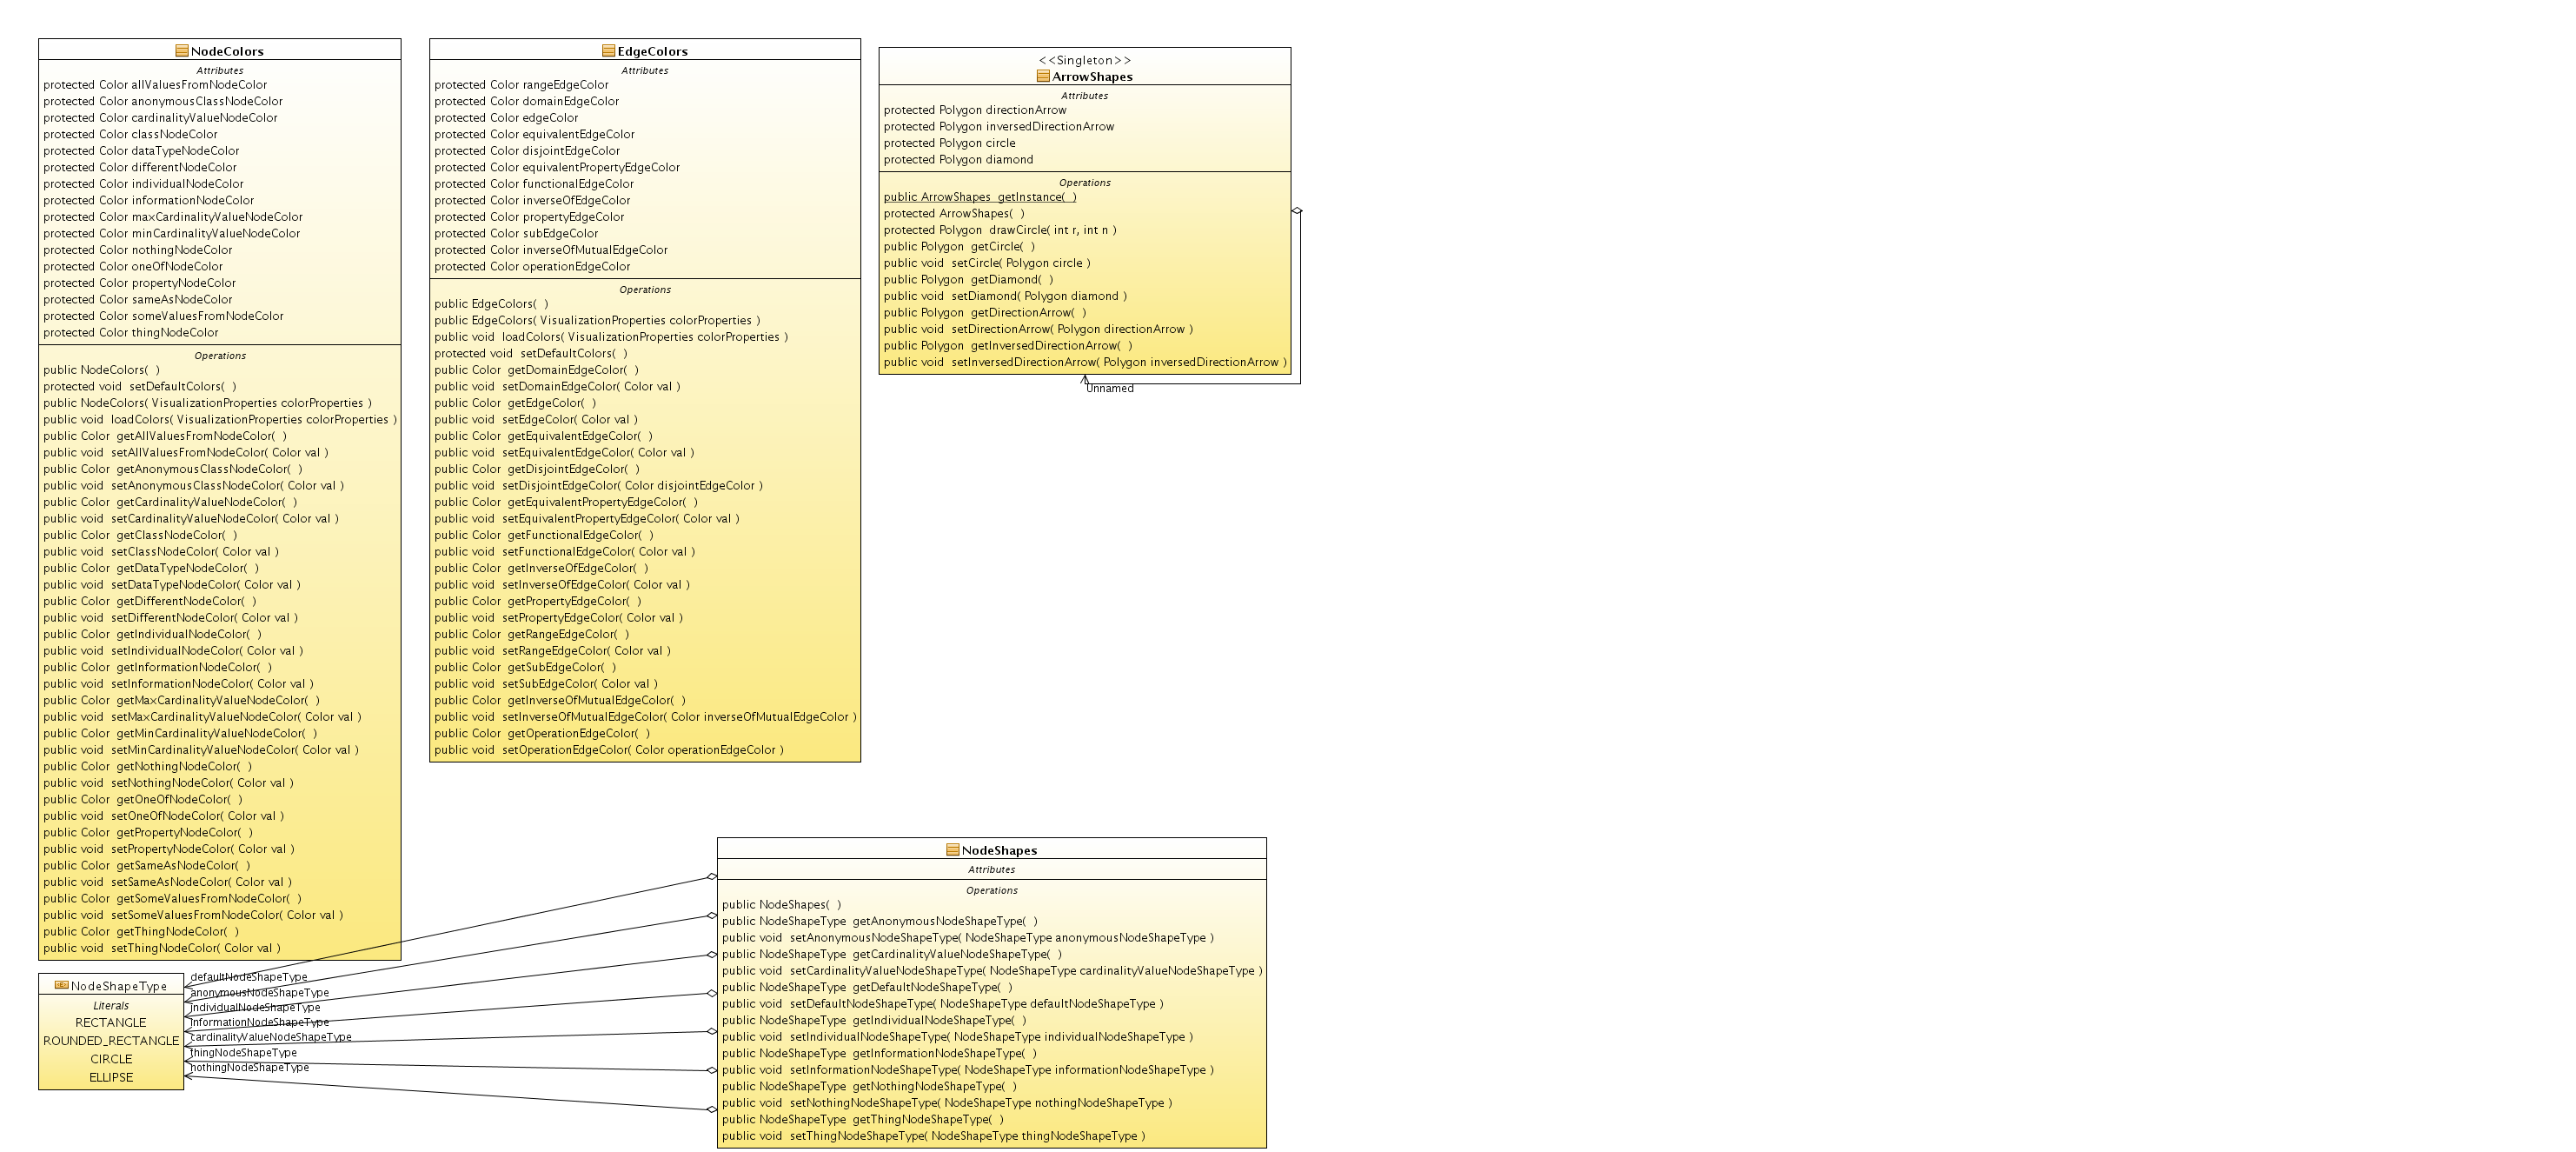
\includegraphics{./modelowanie/OV_UML/OptionsClassDiagram.png}

}

\subsection{Opis klasy}

\begin{center}
 


\begin{longtable}{|m{3cm}|m{9cm}|} \hline

CO001 & EdgeColors \\ \hline
Opis: & Zawiera definicje kolorów dla poszczególnych rodzajów krawędzi.   \\ \hline
Klasy nadrzędne: &     \\ \hline
Atrybuty: & \begin{itemize}
 \item domainEdgeColor
 \item edgeColor
 \item equivalentEdgeColor
 \item equivalentPropertyEdgeColor
 \item functionalEdgeColor
 \item inverseOfEdgeColor
 \item propertyEdgeColor
 \item rangeEdgeColor
 \item subEdgeColor

\end{itemize}
 \\ \hline
Metody: & %\begin{itemize}
% \item 
%\end{itemize}
  \\ \hline
Realizowane wymagania: & WF002 \\ \hline
Priorytet: & średnio ważny \\ \hline

\multicolumn{2}{c}{} \\
 \hline

CO002 & NodeColors \\ \hline
Opis: & Zawiera definicje kolorów dla poszczególnych rodzajów krawędzi.   \\ \hline
Klasy nadrzędne: &     \\ \hline
Atrybuty: & \begin{itemize}
 \item allValuesFromNodeColor
 \item cardinalityNodeColor
 \item cardinalityValueNodeColor
 \item classNodeColor
 \item complementOfNodeColor
 \item dataTypeNodeColor
 \item differentNodeColor
 \item functionalPropertyNodeColor
 \item individualNodeColor
 \item informationNodeColor
 \item intersectionOfNodeColor
 \item inverseFunctionalNodeColor
 \item maxCardinalityValueNodeColor
 \item minCardinalityValueNodeColor
 \item nothingNodeColor
 \item oneOfNodeColor
 \item propertyNodeColor
 \item sameAsNodeColor
 \item someValuesFromNodeColor
 \item symmetricPropertNodeColor
 \item thingNodeColor
 \item transitivePropertyNodeColor
 \item unionOfNodeColor 
\end{itemize}
 \\ \hline
Metody: & %\begin{itemize}
 %\item 
%\end{itemize}
  \\ \hline
Realizowane wymagania: & WF002 \\ \hline
Priorytet: & średnio ważny \\ \hline

%\multicolumn{2}{c}{} \\
% \hline

\end{longtable}


\end{center}

\section{Pakiet nodes}

\subsection{Diagram}

 \scalebox{0.12}{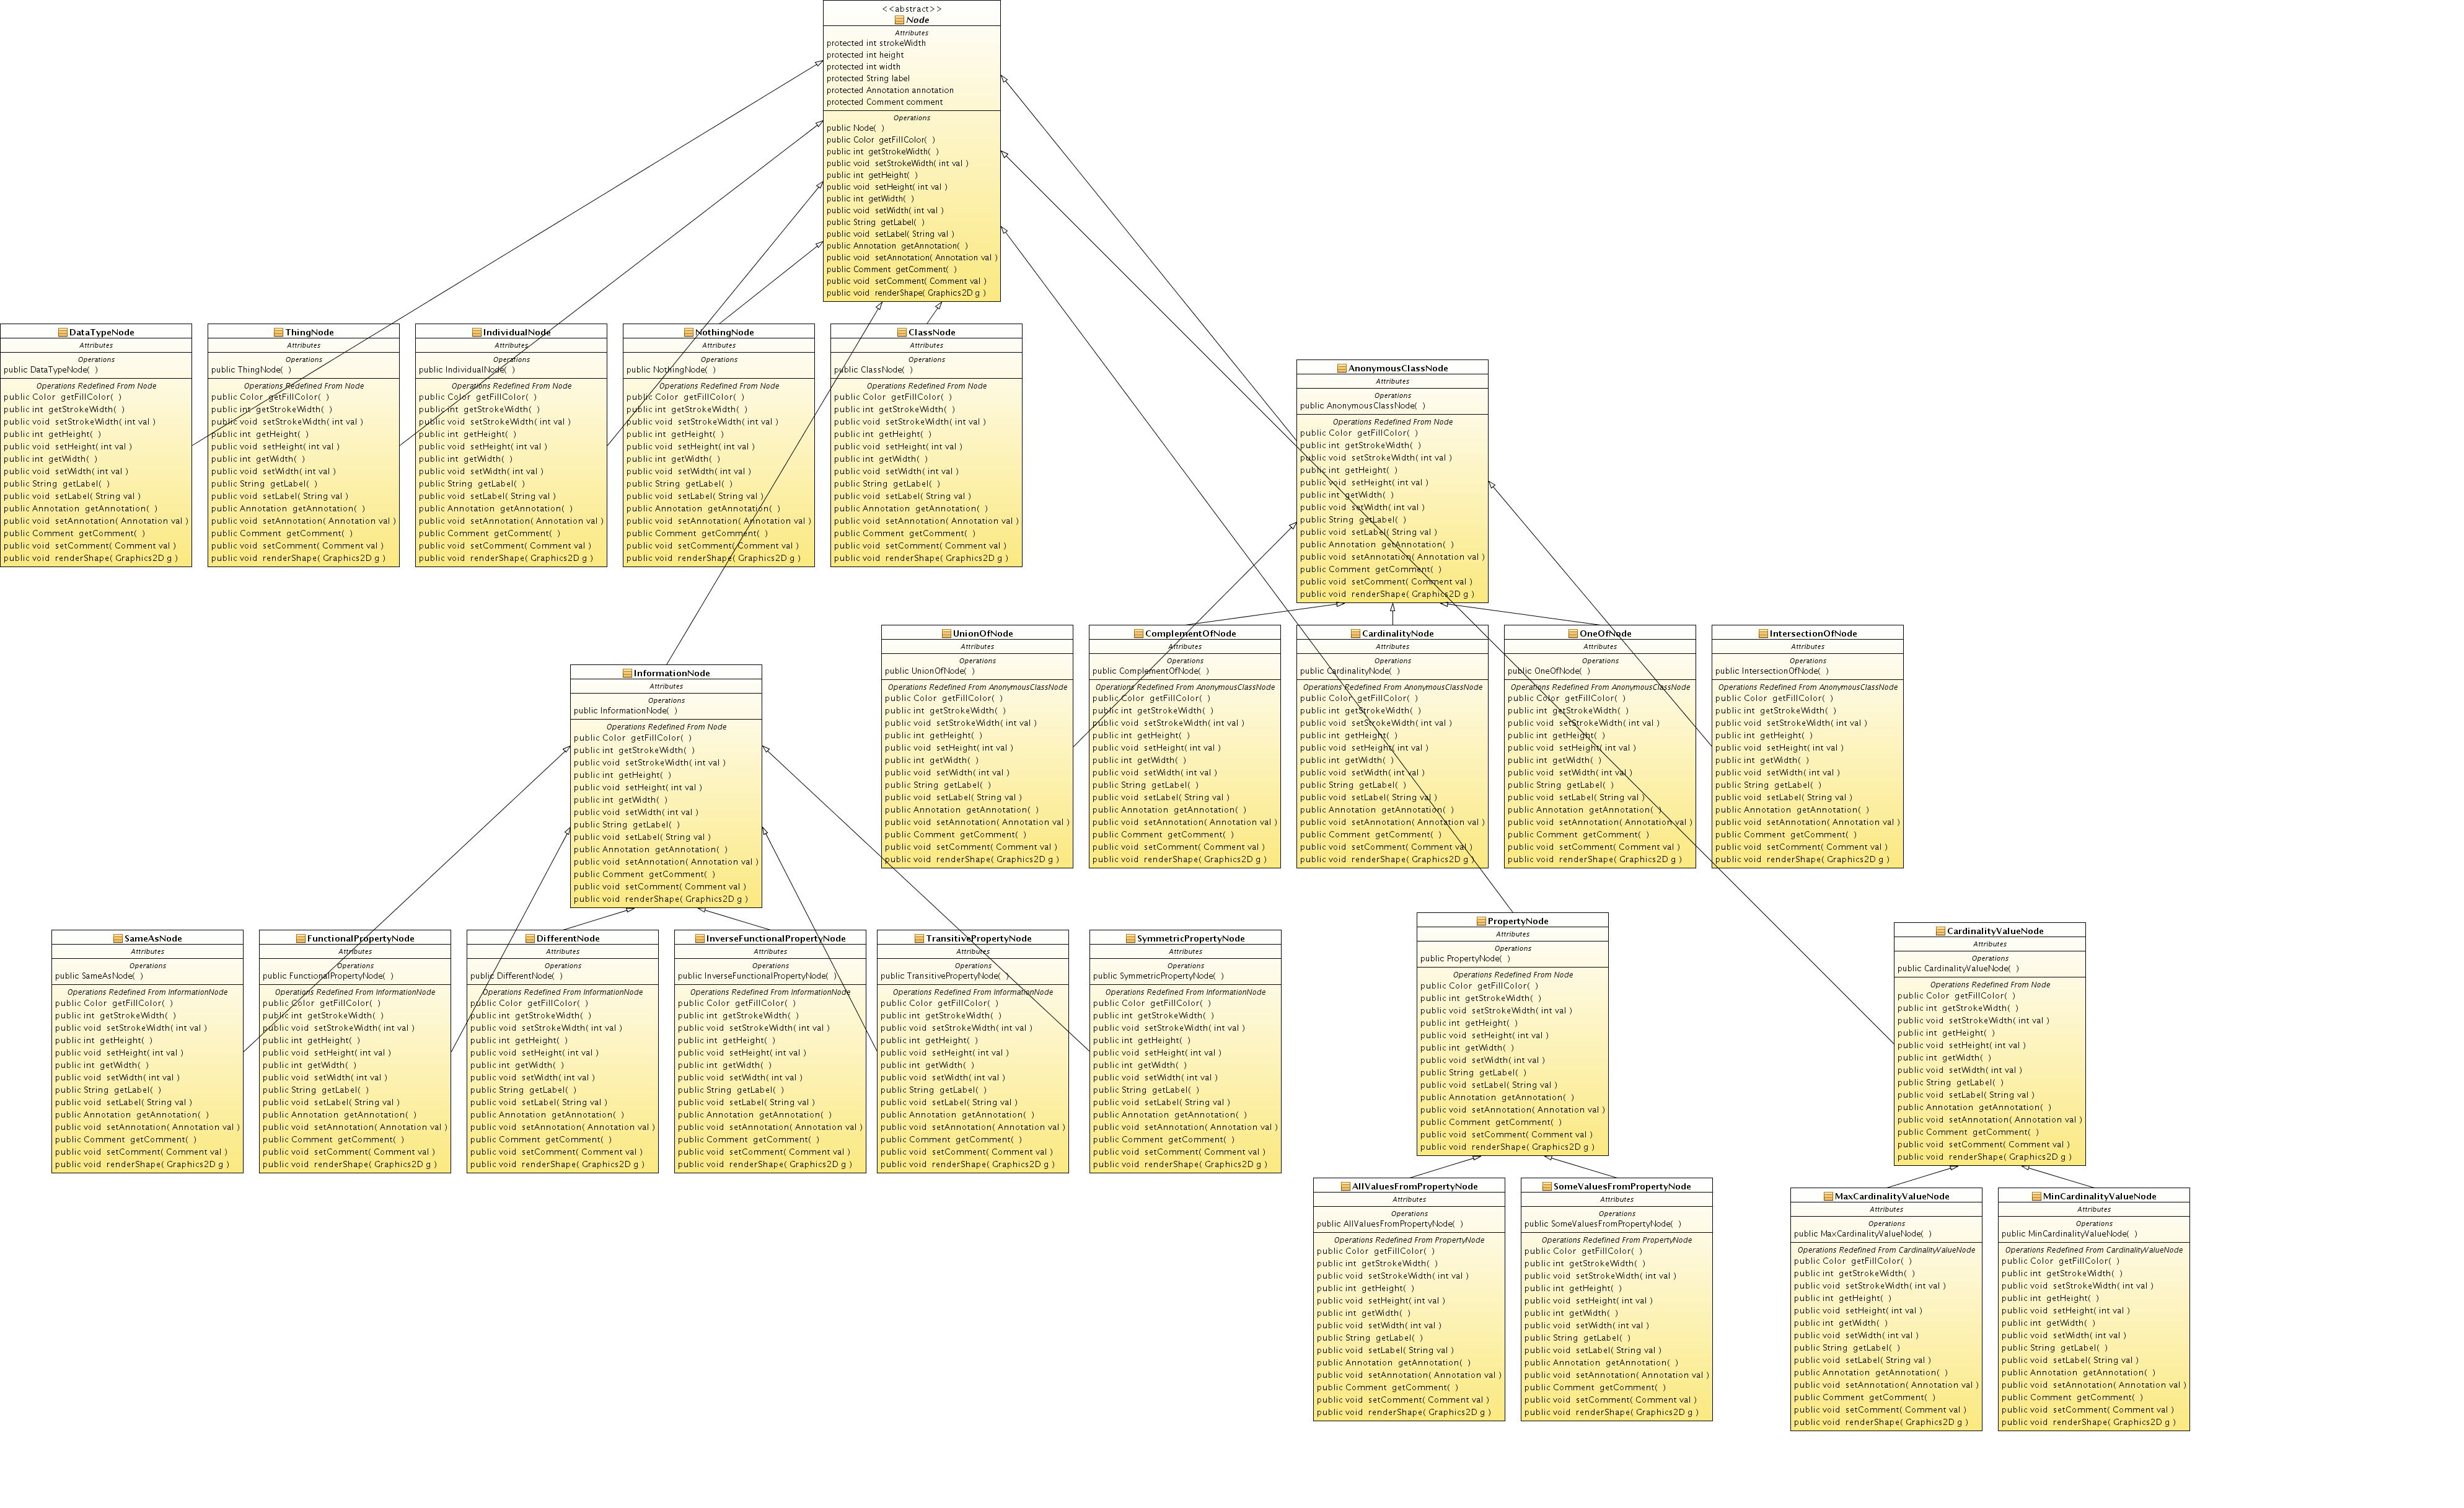
\includegraphics{./modelowanie/OV_UML/NodesClassDiagram.png}}

\subsection{Opis klasy}

\begin{center}
 


\begin{longtable}{|m{3cm}|m{9cm}|} \hline

CN001 & Node \\ \hline
Opis: & Abstrakcyjna klasa - nadrzędna względem wszystkich używanych klas obsługi wierzchołków. Zawiera definicje podstawowych pól o funkcji.    \\ \hline
Klasy nadrzędne: &     \\ \hline
Atrybuty: & \begin{itemize}
 \item strokeWidth
 \item height
 \item width
 \item annotation
 \item comment 
\end{itemize}
 \\ \hline
Metody: & \begin{itemize}
 \item renderShape - metoda wizualizująca dany typ wierzchołka
\end{itemize}
  \\ \hline
Realizowane wymagania: & WF004, WF005, WF006, WF007, WI004 \\ \hline
Priorytet: & bardzo ważne  \\ \hline

\multicolumn{2}{c}{} \\
 \hline

CN002 & AllValuesFromPropertyNode \\ \hline
Opis: &     \\ \hline
Klasy nadrzędne: & Node     \\ \hline
Atrybuty: & 
%\begin{itemize}
 %\item 
%\end{itemize}
 \\ \hline
Metody: & %\begin{itemize}
 %\item 
%\end{itemize}
  \\ \hline
Realizowane wymagania: & WF004, WF006, WF007, WI004 \\ \hline
Priorytet: & ważne \\ \hline

\multicolumn{2}{c}{} \\
 \hline

CN003 & AnonymousClassNode \\ \hline
Opis: &     \\ \hline
Klasy nadrzędne: & Node     \\ \hline
Atrybuty: & %\begin{itemize}
 %\item 
%\end{itemize}
 \\ \hline
Metody: & %\begin{itemize}
 %\item 
%\end{itemize}
  \\ \hline
Realizowane wymagania: & WF005, WI004 \\ \hline
Priorytet: & ważne \\ \hline

\multicolumn{2}{c}{} \\
 \hline

CN004 & CardinalityNode \\ \hline
Opis: &     \\ \hline
Klasy nadrzędne: & AnonymousNode     \\ \hline
Atrybuty: & %\begin{itemize}
 %\item 
%\end{itemize}
 \\ \hline
Metody: & %\begin{itemize}
 %\item 
%\end{itemize}
  \\ \hline
Realizowane wymagania: & WF007, WI004 \\ \hline
Priorytet: & ważne  \\ \hline

\multicolumn{2}{c}{} \\
 \hline

CN005 & CardinalityValueNode \\ \hline
Opis: &     \\ \hline
Klasy nadrzędne: & Node     \\ \hline
Atrybuty: & %\begin{itemize}
 %\item 
%\end{itemize}
 \\ \hline
Metody: & %\begin{itemize}
 %\item 
%\end{itemize}
  \\ \hline
Realizowane wymagania: & WF007, WI004 \\ \hline
Priorytet: & ważne  \\ \hline

\multicolumn{2}{c}{} \\
 \hline

CN006 & ClassNode \\ \hline
Opis: &     \\ \hline
Klasy nadrzędne: & Node     \\ \hline
Atrybuty: & %\begin{itemize}
 %\item 
%\end{itemize}
 \\ \hline
Metody: & %\begin{itemize}
 %\item 
%\end{itemize}
  \\ \hline
Realizowane wymagania: & WF004, WF005, WI004 \\ \hline
Priorytet: & ważne  \\ \hline

\multicolumn{2}{c}{} \\
 \hline

CN007 & ComplementOfNode \\ \hline
Opis: &     \\ \hline
Klasy nadrzędne: & Node     \\ \hline
Atrybuty: & %\begin{itemize}
 %\item 
%\end{itemize}
 \\ \hline
Metody: & %\begin{itemize}
 %\item 
%\end{itemize}
  \\ \hline
Realizowane wymagania: & WF006, WF007, WI004 \\ \hline
Priorytet: & ważne  \\ \hline

\multicolumn{2}{c}{} \\
 \hline

CN008 & DatatypeNode \\ \hline
Opis: &     \\ \hline
Klasy nadrzędne: & Node     \\ \hline
Atrybuty: & %\begin{itemize}
 %\item 
%\end{itemize}
 \\ \hline
Metody: & %\begin{itemize}
 %\item 
%\end{itemize}
  \\ \hline
Realizowane wymagania: & WF004, WI04 \\ \hline
Priorytet: & ważne  \\ \hline

\multicolumn{2}{c}{} \\
 \hline

CN009 & DifferentNode \\ \hline
Opis: &     \\ \hline
Klasy nadrzędne: & Node     \\ \hline
Atrybuty: & %\begin{itemize}
 %\item 
%\end{itemize}
 \\ \hline
Metody: & %\begin{itemize}
 %\item 
%\end{itemize}
  \\ \hline
Realizowane wymagania: & WF006, WF007, WI004 \\ \hline
Priorytet: & ważne  \\ \hline

\multicolumn{2}{c}{} \\
 \hline

CN010 & FunctionalPropertyNode \\ \hline
Opis: &     \\ \hline
Klasy nadrzędne: & InformationNode     \\ \hline
Atrybuty: & %\begin{itemize}
 %\item 
%\end{itemize}
 \\ \hline
Metody: & %\begin{itemize}
 %\item 
%\end{itemize}
  \\ \hline
Realizowane wymagania: & WF006, WF007, WI004 \\ \hline
Priorytet: & ważne  \\ \hline

\multicolumn{2}{c}{} \\
 \hline

CN011 & IndividualNode \\ \hline
Opis: &     \\ \hline
Klasy nadrzędne: & Node     \\ \hline
Atrybuty: & %\begin{itemize}
 %\item 
%\end{itemize}
 \\ \hline
Metody: & %\begin{itemize}
 %\item 
%\end{itemize}
  \\ \hline
Realizowane wymagania: & WF004, WI004 \\ \hline
Priorytet: & ważne  \\ \hline

\multicolumn{2}{c}{} \\
 \hline

CN012 & InformationNode \\ \hline
Opis: &     \\ \hline
Klasy nadrzędne: & Node     \\ \hline
Atrybuty: & %\begin{itemize}
 %\item 
%\end{itemize}
 \\ \hline
Metody: & %\begin{itemize}
 %\item 
%\end{itemize}
  \\ \hline
Realizowane wymagania: & WF010, WI004 \\ \hline
Priorytet: & ważne  \\ \hline

\multicolumn{2}{c}{} \\
 \hline

CN013 & IntersectionOfNode \\ \hline
Opis: &     \\ \hline
Klasy nadrzędne: & AnonymousNode     \\ \hline
Atrybuty: & %\begin{itemize}
 %\item 
%\end{itemize}
 \\ \hline
Metody: & %\begin{itemize}
 %\item 
%\end{itemize}
  \\ \hline
Realizowane wymagania: & WF005, WI004 \\ \hline
Priorytet: & ważne  \\ \hline

\multicolumn{2}{c}{} \\
 \hline

CN014 & inverseFunciotnalPropertyNode \\ \hline
Opis: &     \\ \hline
Klasy nadrzędne: & InformationNode     \\ \hline
Atrybuty: & %\begin{itemize}
 %\item 
%\end{itemize}
 \\ \hline
Metody: & %\begin{itemize}
 %\item 
%\end{itemize}
  \\ \hline
Realizowane wymagania: & WF007, WI004 \\ \hline
Priorytet: & ważne  \\ \hline

\multicolumn{2}{c}{} \\
 \hline

CN015 & MaxCardinalityValueNode \\ \hline
Opis: &     \\ \hline
Klasy nadrzędne: & CardinalityValueNode     \\ \hline
Atrybuty: & %\begin{itemize}
 %\item 
%\end{itemize}
 \\ \hline
Metody: & %\begin{itemize}
 %\item 
%\end{itemize}
  \\ \hline
Realizowane wymagania: & WF007, WI004 \\ \hline
Priorytet: & ważne  \\ \hline

\multicolumn{2}{c}{} \\
 \hline

CN016 & MinCardinalityValueNode \\ \hline
Opis: &     \\ \hline
Klasy nadrzędne: & CardinalityValueNode     \\ \hline
Atrybuty: & %\begin{itemize}
 %\item 
%\end{itemize}
 \\ \hline
Metody: & %\begin{itemize}
 %\item 
%\end{itemize}
  \\ \hline
Realizowane wymagania: & WF007, WI004 \\ \hline
Priorytet: & ważne  \\ \hline

\multicolumn{2}{c}{} \\
 \hline

CN017 & NothingNode \\ \hline
Opis: &     \\ \hline
Klasy nadrzędne: & Node     \\ \hline
Atrybuty: & %\begin{itemize}
 %\item 
%\end{itemize}
 \\ \hline
Metody: & %\begin{itemize}
 %\item 
%\end{itemize}
  \\ \hline
Realizowane wymagania: & WF004, WF005, WI004 \\ \hline
Priorytet: & ważne  \\ \hline

\multicolumn{2}{c}{} \\
 \hline

CN018 & OneOfNode \\ \hline
Opis: &     \\ \hline
Klasy nadrzędne: & AnonymousClassNode     \\ \hline
Atrybuty: & %\begin{itemize}
 %\item 
%\end{itemize}
 \\ \hline
Metody: & %\begin{itemize}
 %\item 
%\end{itemize}
  \\ \hline
Realizowane wymagania: & WF005, WF006, WI004 \\ \hline
Priorytet: & ważne  \\ \hline

\multicolumn{2}{c}{} \\
 \hline

CN019 & PropertyNode \\ \hline
Opis: &     \\ \hline
Klasy nadrzędne: & Node     \\ \hline
Atrybuty: & %\begin{itemize}
 %\item 
%\end{itemize}
 \\ \hline
Metody: & %\begin{itemize}
 %\item 
%\end{itemize}
  \\ \hline
Realizowane wymagania: & WF004, WF007, WI004 \\ \hline
Priorytet: & ważne  \\ \hline

\multicolumn{2}{c}{} \\
 \hline

CN020 & SameAsNode \\ \hline
Opis: &     \\ \hline
Klasy nadrzędne: & InformationNode     \\ \hline
Atrybuty: & %\begin{itemize}
 %\item 
%\end{itemize}
 \\ \hline
Metody: & %\begin{itemize}
 %\item 
%\end{itemize}
  \\ \hline
Realizowane wymagania: & WF005, WF006, WI004 \\ \hline
Priorytet: & ważne  \\ \hline

\multicolumn{2}{c}{} \\
 \hline

CN021 & SomeValuesFromPropertyNode \\ \hline
Opis: &     \\ \hline
Klasy nadrzędne: & PropertyNode     \\ \hline
Atrybuty: & %\begin{itemize}
 %\item 
%\end{itemize}
 \\ \hline
Metody: & %\begin{itemize}
 %\item 
%\end{itemize}
  \\ \hline
Realizowane wymagania: & WF005, WF006, WI004 \\ \hline
Priorytet: & ważne  \\ \hline

\multicolumn{2}{c}{} \\
 \hline

CN022 & SymmetricPropertNode \\ \hline
Opis: &     \\ \hline
Klasy nadrzędne: & InformationNode     \\ \hline
Atrybuty: & %\begin{itemize}
 %\item 
%\end{itemize}
 \\ \hline
Metody: & %\begin{itemize}
 %\item 
%\end{itemize}
  \\ \hline
Realizowane wymagania: & WF007, WI004 \\ \hline
Priorytet: & ważne  \\ \hline

\multicolumn{2}{c}{} \\
 \hline

CN023 & ThingNode \\ \hline
Opis: &     \\ \hline
Klasy nadrzędne: & Node     \\ \hline
Atrybuty: & %\begin{itemize}
 %\item 
%\end{itemize}
 \\ \hline
Metody: & %\begin{itemize}
 %\item 
%\end{itemize}
  \\ \hline
Realizowane wymagania: & WF004, WF005, WI004 \\ \hline
Priorytet: & ważne  \\ \hline

\multicolumn{2}{c}{} \\
 \hline

CN024 & TreansitivePropertyNode \\ \hline
Opis: &     \\ \hline
Klasy nadrzędne: & InformationNode     \\ \hline
Atrybuty: & %\begin{itemize}
 %\item 
%\end{itemize}
 \\ \hline
Metody: & %\begin{itemize}
 %\item 
%\end{itemize}
  \\ \hline
Realizowane wymagania: & WF006, WF007, WI004 \\ \hline
Priorytet: & ważne  \\ \hline

\multicolumn{2}{c}{} \\
 \hline

CN025 & UnionOfNode \\ \hline
Opis: &     \\ \hline
Klasy nadrzędne: & AnonymousNode     \\ \hline
Atrybuty: & %\begin{itemize}
 %\item 
%\end{itemize}
 \\ \hline
Metody: & %\begin{itemize}
 %\item 
%\end{itemize}
  \\ \hline
Realizowane wymagania: & WF005, WF006, WI004 \\ \hline
Priorytet: & ważne  \\ \hline

%\multicolumn{2}{c}{} \\
% \hline


\end{longtable}

\end{center}

\section{Pakiet edges}

\subsection{Diagram}

 \scalebox{0.26}{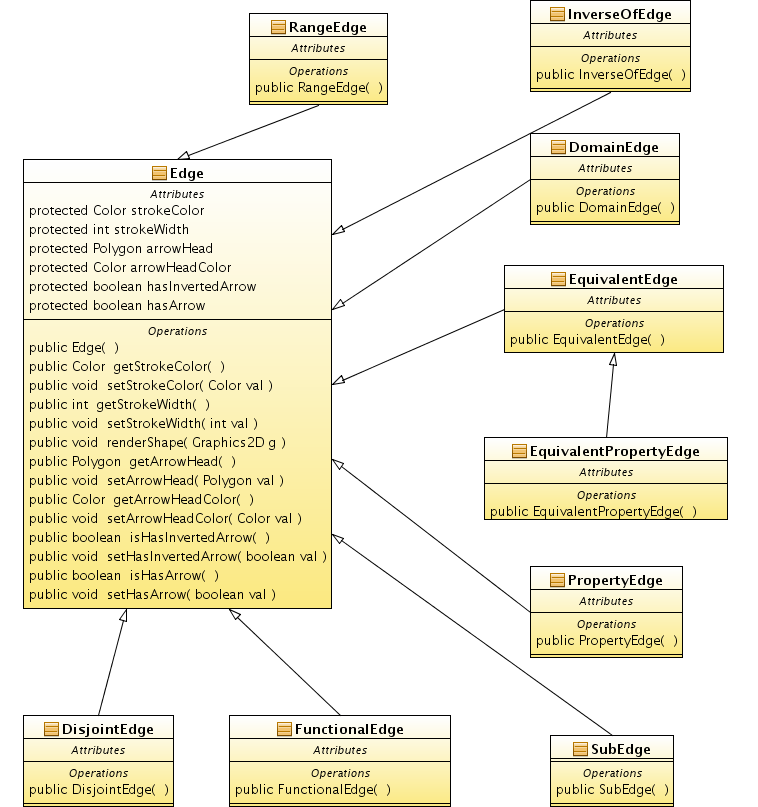
\includegraphics{./modelowanie/OV_UML/EdgeClassDiagram.png}}

\subsection{Opis klasy}

\begin{center}

\begin{longtable}{|m{3cm}|m{9cm}|} \hline

CE001 &  \\ \hline
Opis: & Edge    \\ \hline
Klasy nadrzędne: &     \\ \hline
Atrybuty: & \begin{itemize}
 \item strokeColor
 \item strokeWidth 
\end{itemize}
 \\ \hline
Metody: & \begin{itemize}
 \item renderShape(Graphics2D g)
\end{itemize}
  \\ \hline
Realizowane wymagania: & WF006, WF007, WI004 \\ \hline
Priorytet: & bardzo ważne  \\ \hline

\multicolumn{2}{c}{} \\
 \hline

CE002 &  \\ \hline
Opis: & DisjointEdge    \\ \hline
Klasy nadrzędne: & Edge    \\ \hline
Atrybuty: & %\begin{itemize}
 %\item 
%\end{itemize}
 \\ \hline
Metody: & %\begin{itemize}
 %\item 
%\end{itemize}
  \\ \hline
Realizowane wymagania: & WF006, WF007, WI004 \\ \hline
Priorytet: & ważne  \\ \hline

\multicolumn{2}{c}{} \\
 \hline

CE003 &  \\ \hline
Opis: & DomainEdge    \\ \hline
Klasy nadrzędne: & Edge    \\ \hline
Atrybuty: & %\begin{itemize}
 %\item 
%\end{itemize}
 \\ \hline
Metody: & %\begin{itemize}
 %\item 
%\end{itemize}
  \\ \hline
Realizowane wymagania: & WF006, WF007, WI004 \\ \hline
Priorytet: & ważne  \\ \hline

\multicolumn{2}{c}{} \\
 \hline

CE004 &  \\ \hline
Opis: & EquivalentEdge    \\ \hline
Klasy nadrzędne: & Edge    \\ \hline
Atrybuty: & %\begin{itemize}
 %\item 
%\end{itemize}
 \\ \hline
Metody: & %\begin{itemize}
 %\item 
%\end{itemize}
  \\ \hline
Realizowane wymagania: & WF006, WF007, WI004 \\ \hline
Priorytet: & ważne  \\ \hline

\multicolumn{2}{c}{} \\
 \hline

CE005 &  \\ \hline
Opis: & EquivalentPropertyEdge    \\ \hline
Klasy nadrzędne: & EquivalentEdge    \\ \hline
Atrybuty: & %\begin{itemize}
 %\item 
%\end{itemize}
 \\ \hline
Metody: & %\begin{itemize}
 %\item 
%\end{itemize}
  \\ \hline
Realizowane wymagania: & WF006, WF007, WI004 \\ \hline
Priorytet: & ważne  \\ \hline

\multicolumn{2}{c}{} \\
 \hline

CE006 &  \\ \hline
Opis: & FunctionaltEdge    \\ \hline
Klasy nadrzędne: & Edge    \\ \hline
Atrybuty: & %\begin{itemize}
 %\item 
%\end{itemize}
 \\ \hline
Metody: & %\begin{itemize}
 %\item 
%\end{itemize}
  \\ \hline
Realizowane wymagania: & WF006, WF007, WI004 \\ \hline
Priorytet: & ważne  \\ \hline

\multicolumn{2}{c}{} \\
 \hline

CE007 &  \\ \hline
Opis: & InverseOfEdge    \\ \hline
Klasy nadrzędne: & Edge    \\ \hline
Atrybuty: & %\begin{itemize}
 %\item 
%\end{itemize}
 \\ \hline
Metody: & %\begin{itemize}
 %\item 
%\end{itemize}
  \\ \hline
Realizowane wymagania: & WF006, WF007, WI004 \\ \hline
Priorytet: & ważne  \\ \hline

\multicolumn{2}{c}{} \\
 \hline

CE008 &  \\ \hline
Opis: & PropertyEdge    \\ \hline
Klasy nadrzędne: & Edge    \\ \hline
Atrybuty: & %\begin{itemize}
 %\item 
%\end{itemize}
 \\ \hline
Metody: & %\begin{itemize}
 %\item 
%\end{itemize}
  \\ \hline
Realizowane wymagania: & WF006, WF007, WI004 \\ \hline
Priorytet: & ważne  \\ \hline

\multicolumn{2}{c}{} \\
 \hline

CE009 &  \\ \hline
Opis: & RangeEdge    \\ \hline
Klasy nadrzędne: & Edge    \\ \hline
Atrybuty: & %\begin{itemize}
 %\item 
%\end{itemize}
 \\ \hline
Metody: & %\begin{itemize}
 %\item 
%\end{itemize}
  \\ \hline
Realizowane wymagania: & WF006, WF007, WI004 \\ \hline
Priorytet: & ważne  \\ \hline

\multicolumn{2}{c}{} \\
 \hline

CE010 &  \\ \hline
Opis: & SubEdge    \\ \hline
Klasy nadrzędne: & Edge    \\ \hline
Atrybuty: & %\begin{itemize}
 %\item 
%\end{itemize}
 \\ \hline
Metody: & %\begin{itemize}
 %\item 
%\end{itemize}
  \\ \hline
Realizowane wymagania: & WF006, WF007, WI004 \\ \hline
Priorytet: & ważne  \\ \hline

%\multicolumn{2}{c}{} \\
% \hline


\end{longtable}

\end{center}

\section{Pakiet visualization }

\subsection{Diagram}

 \scalebox{0.45}{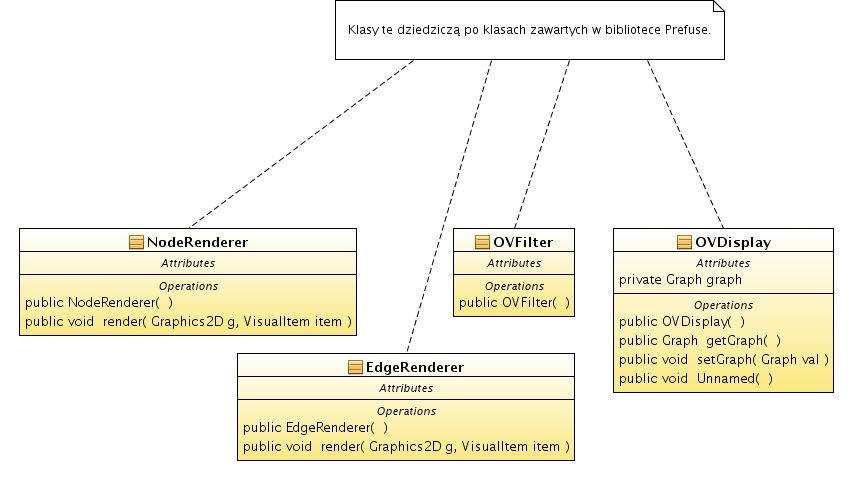
\includegraphics{./modelowanie/OV_UML/VisualizationClassDiagram.png}}

\subsection{Opis klasy}

\begin{center}
 

\begin{longtable}{|m{3cm}|m{9cm}|} \hline

CV001 & EdgeRenderer \\ \hline
Opis: & Klasa przeciążająca metody renderowania krawędzi grafu z biblioteki prefuse. \\ \hline
Klasy nadrzędne: &  prefuse.render.EdgeRenderer   \\ \hline
Atrybuty: & %\begin{itemize}
 %\item 
%\end{itemize}
 \\ \hline
Metody: & \begin{itemize}
 \item Render - metoda renderująca krawędź
\end{itemize}
  \\ \hline
Realizowane wymagania: & WF001, WF008, WI004 \\ \hline
Priorytet: & ważne  \\ \hline

\multicolumn{2}{c}{} \\
 \hline

CV002 & NodeRenderer \\ \hline
Opis: & Klasa przeciążająca metody renderowania wierzchołków grafu z biblioteki prefuse.    \\ \hline
Klasy nadrzędne: &  prefuse.render.LabelRenderer   \\ \hline
Atrybuty: & %\begin{itemize}
 %\item 
%\end{itemize}
 \\ \hline
Metody: & \begin{itemize}
 \item Render - metoda renderująca wierzchołek
\end{itemize}
  \\ \hline
Realizowane wymagania: & WF001, WF008, WI004 \\ \hline
Priorytet: & ważne  \\ \hline

\multicolumn{2}{c}{} \\
 \hline

CV003 & OVDisplay \\ \hline
Opis: &     \\ \hline
Klasy nadrzędne: &  prefuse.Display   \\ \hline
Atrybuty: & %\begin{itemize}
 %\item 
%\end{itemize}
 \\ \hline
Metody: & %\begin{itemize}
 %\item 
%\end{itemize}
  \\ \hline
Realizowane wymagania: & WF001, WF002, WF008, WI004 \\ \hline
Priorytet: & ważne  \\ \hline

\multicolumn{2}{c}{} \\
 \hline

CV004 & OVRender \\ \hline
Opis: &     \\ \hline
Klasy nadrzędne: &  ???   \\ \hline
Atrybuty: & %\begin{itemize}
 %\item 
%\end{itemize}
 \\ \hline
Metody: & %\begin{itemize}
 %\item 
%\end{itemize}
  \\ \hline
Realizowane wymagania: & WF001, WF008, WI004 \\ \hline
Priorytet: & ważne  \\ \hline

%\multicolumn{2}{c}{} \\
% \hline


\end{longtable}

\end{center}

\section{Pakiet graph}

\subsection{Diagram}

 \scalebox{0.6}{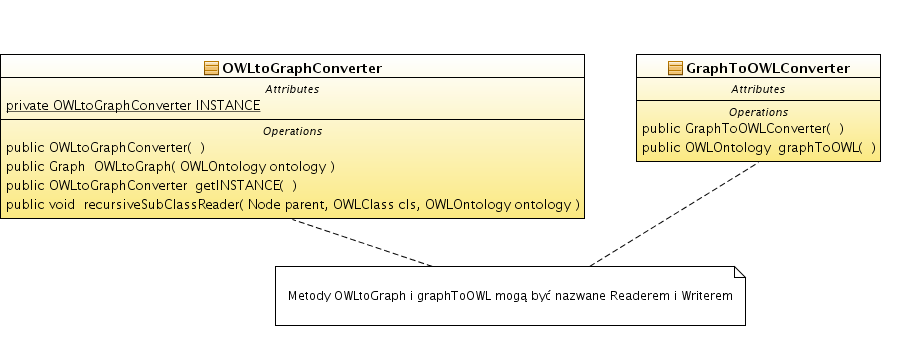
\includegraphics{./modelowanie/OV_UML/GraphClassDiagram.png}}

\subsection{Opis klasy}

\begin{center}
 


\begin{longtable}{|m{3cm}|m{9cm}|} \hline

CG001 & GraphToOWLConverter \\ \hline
Opis: & Klasa zawierająca metody pozwalające na przetwarzanie obiektów grafów z prefuse na obiekty OWL API. \\ \hline
Klasy nadrzędne: &     \\ \hline
Atrybuty: & %\begin{itemize}
 %\item 
%\end{itemize}
 \\ \hline
Metody: & \begin{itemize}
 \item GraphToOWL
\end{itemize}
  \\ \hline
Realizowane wymagania: & WD001, WI004 \\ \hline
Priorytet: & ważne  \\ \hline

\multicolumn{2}{c}{} \\
 \hline

CG002 & OWLtoGraphConverter \\ \hline
Opis: & Klasa zawierająca metody pozwalające na przetwarzanie obiektów OWL API na obiekty prefuse. \\ \hline
Klasy nadrzędne: &     \\ \hline
Atrybuty: & %\begin{itemize}
 %\item 
%\end{itemize}
 \\ \hline
Metody: & \begin{itemize}
 \item OWLtoGraph
\end{itemize}
  \\ \hline
Realizowane wymagania: & WD001, WI004 \\ \hline
Priorytet: & ważne  \\ \hline

%\multicolumn{2}{c}{} \\
% \hline


\end{longtable}

\end{center}


%\clearpage
%\phantomsection
%\addcontentsline{toc}{section}{Literatura}
%\bibliography{biblio}

\end{document}
